\chapter*{Capítulo 2 \vspace{0.5cm} \break Desarrollo del nuevo sistema de capacitación}
\setcounter{chapter}{2}
\setcounter{section}{0}
\addcontentsline{toc}{chapter}{Capítulo 2: Desarrollo del nuevo sistema de capacitación}

Para que el desarrollo de un proyecto concluya con éxitos, primero debe realizarse el diseño de lo que se pretende obtener, así como analizar los requisitos que se deben cumplir. En este capítulo se presentan los diagramas utilizados en la elaboración del nuevo sistema de capacitación, así como la estructura que posee, sus principales funcionalidades y algunas comparaciones con el modelo del sistema SECPROIT.

\section{Descripción del negocio}
Lo que se pretende conseguir con este nuevo sistema es rectificar las limitaciones existentes en el SECPROIT actual. Para ello, el sistema debe satisfacer el objetivo principal del software anterior: capacitar a los operarios ante los procesos productivos de una fábrica.
Partiendo de esta premisa, la solución debe poseer un modelo de entrenamiento que ponga a prueba a los operarios de la industria. También debe contar con un administrador que sea el responsable de incluir a los usuarios y las áreas.

A la hora de realizar el entrenamiento, se deben evaluar tres etapas fundamentales: variables, causas y recomendaciones. Si el trabajador logra superar estas etapas, puede darse por aprobado el entrenamiento de ese proceso.

\subsection{Modelo de dominio}
Un modelo de dominio es la representación de las clases conceptuales del mundo real, no de componentes de software. Su utilidad radica en ser una forma de inspiración para el diseño de entidades. Es el artefacto clave en el análisis orientado a objetos \cite{Herchi2012}.

El modelo de dominio de este sistema (\textsl{Figura \ref{fig:dominio}}) no es muy diferente del modelo del sistema SECPROIT. Para representarlo se tuvieron en cuenta tres colores, con el objetivo de diferenciar los cambios realizados:

\begin{itemize}
\item \textbf{Azul}: representa aquellas entidades que no sufrieron ningún cambio significativo con respecto al sistema SECPROIT
\item \textbf{Amarillo}: representa aquellas entidades que fueron modificadas, pero que siguen cumpliendo las mismas funciones
\item \textbf{Verde}: representa las entidades que son totalmente nuevas
\end{itemize}

\begin{figure}[h]
\centering
 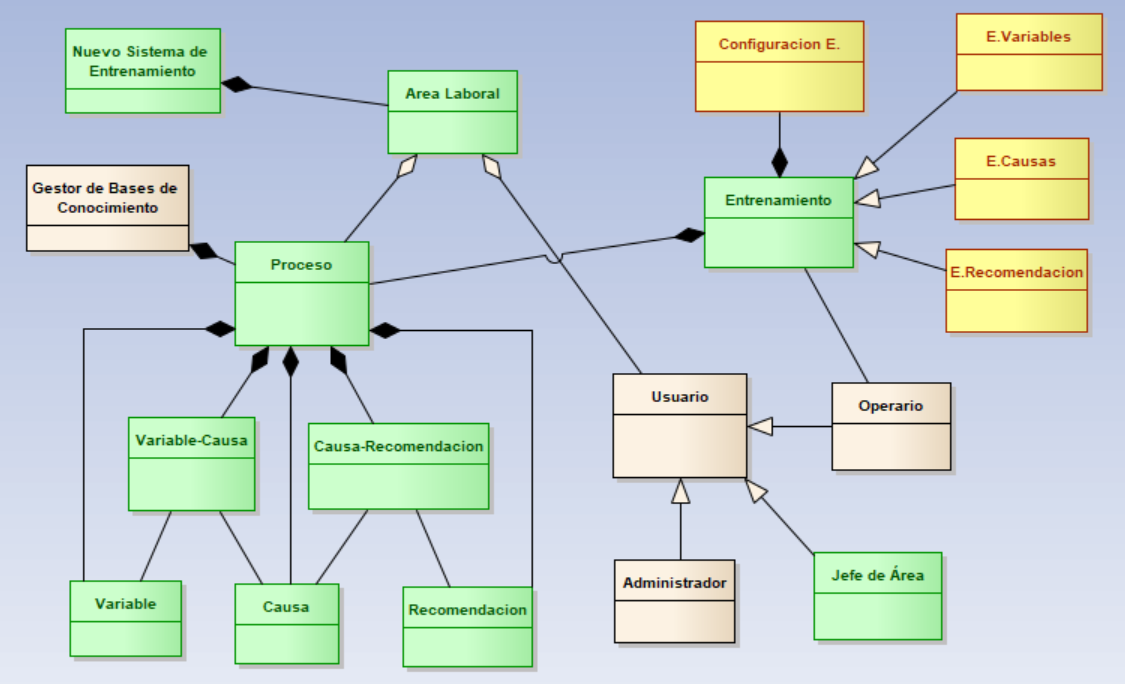
\includegraphics[width=0.7\linewidth]{imagen/dominio.png}
 \caption{Modelo de dominio}
 \label{fig:dominio} 
\end{figure}

Las entidades que contienen algunos cambios (\textsl{Tabla \ref{tab:ent-amarilla}}), indican que también se realizaron arreglos en las estructuras que estas seguían, es decir, variaciones en la base de datos y en las clases del sistema.

\begin{table}[H]
\begin{center}
\begin{tabular}{ | c | p{5cm} |  p{5.2cm} | }
\hline
\textbf{Entidad} & \textbf{Descripción} & \textbf{Cambios}\\
\hline
Sistema SECPROIT & Representa el sistema & Cambian las clases que posee \\
\hline
Jefe de área & Es un tipo de usuario y se encarga de administrar los procesos & Antes era especialista y solo creaba los procesos \\
\hline
Proceso & Representa los procesos & Se le agrega un nuevo atributo: configuración de entrenamiento \\
\hline
Entrenamiento & Representa el entrenamiento del usuario & Se le agrega nuevos intentos por cada etapa \\
\hline
\end{tabular}
\caption{Modelo de dominio: entidades que sufrieron cambios}
\label{tab:ent-amarilla}
\end{center}
\end{table}

La entidades que no fueron modificadas (\textsl{Tabla \ref{tab:ent-azul}}),  no sufrieron cambios porque, basadas en las tareas que desempeñan, no varían sus funciones en este nuevo modelo.

\begin{table}[H]
\begin{center}
\begin{tabular}{ | c | p{12cm} | }
\hline
\textbf{Entidad} & \textbf{Descripción} \\
\hline
Área & Representa el lugar donde laboran los trabajadores y es donde están presentes los procesos \\
\hline
Usuario & Representa a la persona que va interactuar con el sistema \\
\hline
Administrador & Es un tipo de usuario y se encarga de administrar las entidades del sistema (áreas y demás usuarios) \\
\hline
Operario & Es un tipo de usuario y se encarga de realizar los entrenamientos \\
\hline
Base de datos & Representa el archivo \textsf{anm} \\
\hline
Base de reglas & Representa el archivo \textsf{drl} \\
\hline
Drools & Es la entidad que permite ejecutar las reglas del proceso \\
\hline
Variable & Forma parte de la base de datos del proceso y contiene la información que se se evalúa en la primera etapa \\
\hline
Causa & Forma parte de la base de datos del proceso y contiene la información que se evalúa en la segunda etapa \\
\hline
Recm. & Forma parte de la base de datos del proceso, representa las recomendaciones y contiene la información que se evalúa en la tercera etapa \\
\hline
Variable-Causa & Forma parte de la base de reglas del proceso y contiene la información que se evalúa en la primera y segunda etapa \\
\hline
Causa-Recm. & Forma parte de la base de reglas del proceso y contiene la información que se evalúa en la tercera etapa \\
\hline
\end{tabular}
\caption{Modelo de dominio: entidades que no sufrieron cambios}
\label{tab:ent-azul}
\end{center}
\end{table}

Por último, las entidades nuevas (\textsl{Tabla \ref{tab:ent-verde}}) son clases que fueron incluidas con el fin de enmendar alguna limitación.

\begin{table}[H]
\begin{center}
\begin{tabular}{ | c | p{12cm} | }
\hline
\textbf{Entidad} & \textbf{Descripción} \\
\hline
Configuración & Es la configuración del entrenamiento de un proceso, es decir, un grupo de características determinadas en el entrenamiento \\
\hline
Etapas & Representa las etapas del entrenamiento \\
\hline
E-Variable & Es la primera etapa, donde se evalúan las variables \\
\hline
E-Causa & Es la segunda etapa, donde se evalúan las causas \\
\hline
E-Recm. & Es la tercera etapa, donde se evalúan las recomendaciones \\
\hline
\end{tabular}
\caption{Modelo de dominio: entidades nuevas}
\label{tab:ent-verde}
\end{center}
\end{table}

\subsection{Reglas del negocio}
Las reglas de un negocio son directrices y restricciones que ayudan a regular las operaciones de una entidad determinada. Para cada proceso existen reglas que deben seguirse durante la ejecución, ya que estas ayudan a definir \textbf{cómo} deben realizarse las tareas, por \textbf{quién}, \textbf{cuándo}, \textbf{dónde} y \textbf{por qué} \cite{Chisholm2007}. A modo de resumen, las reglas de un negocio son límites impuestos a las operaciones para que estén en sintonía con las políticas y objetivos de la institución.

En el sistema SECPROIT existen un conjunto de reglas primordiales que no se deben dejar de cumplir:
\begin{itemize}
\item Cada usuario debe poseer un único rol
\item Para poder introducir un nuevo usuario debe existir, al menos, un área laboral
\item Un usuario no puede pertenecer a más de un área
\item Solo puede existir un jefe de área por área
\item Para poder introducir un nuevo proceso debe existir, al menos, un área laboral
\item Un proceso no puede pertenecer a más de un área
\item Para generar un nuevo entrenamiento debe existir, al menos, un usuario que cumpla el rol de operario y un proceso que sea de la misma área
\item Para entrenar en la etapa de las causas debe haberse aprobado la etapa de las variables
\item Para entrenar en la etapa de las recomendaciones debe haberse aprobado la etapa de las causas
\item Los usuarios con rol de administrador son los únicos que pueden gestionar las áreas y las cuentas de los usuarios
\item No se puede eliminar la cuenta de un usuario
\item Los usuarios con rol de jefe de área son los únicos que pueden gestionar los procesos de sus áreas y configurar los entrenamientos
\item Los usuarios con rol de operario son los únicos que pueden entrenar
\item Para superar un entrenamiento se deben haber aprobado las tres etapas (variables, causas y recomendaciones)
\end{itemize}

\subsection{Diagrama de actividades}
El Lenguaje Unificado de Modelado (UML) incluye varios subconjuntos de modelos, entre los que se encuentran los diagramas de actividades. Estos diagramas son considerados diagramas de comportamiento, porque describen el comportamiento del sistema que representan \cite{Eriksson2000}.

En el diagrama de actividades del nuevo sistema de capacitación (\textsl{Figura \ref{fig:actividades}}) se pueden observar tres colores: azul, amarillo y verde. El color azul indica que el flujo funciona de la misma manera que en el SECPROIT, el color amarillo representa un ligero cambio y el verde, representa una acción totalmente nueva.

\begin{figure}[h]
\centering
 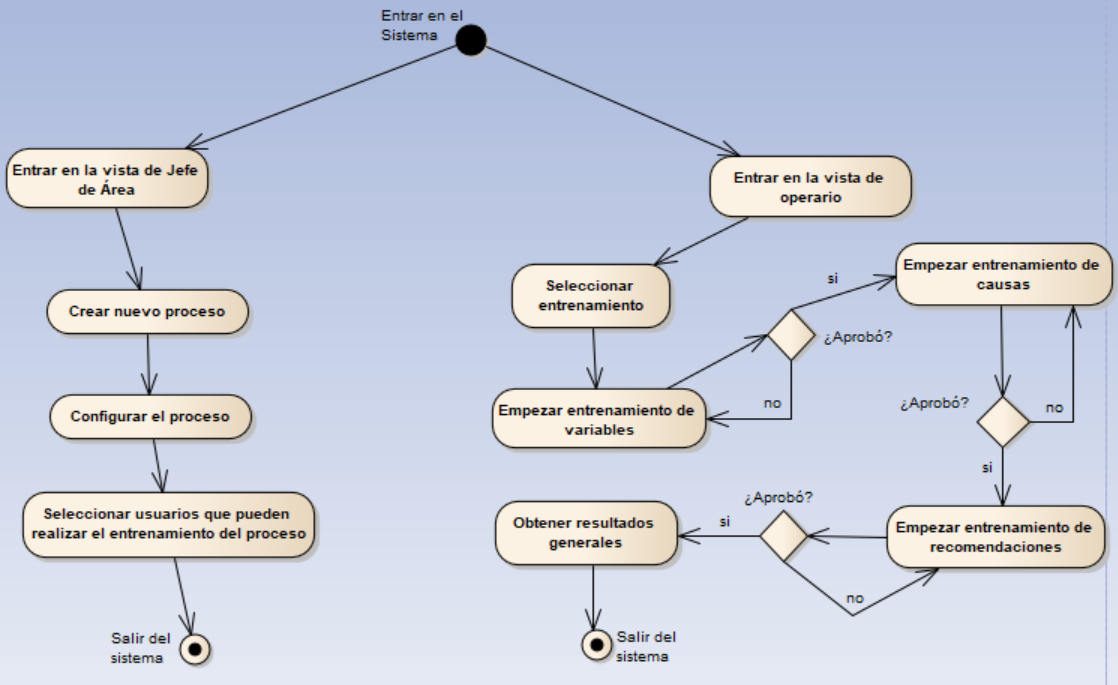
\includegraphics[width=0.65\linewidth]{imagen/actividades.png}
 \caption{Diagrama de actividades}
 \label{fig:actividades} 
\end{figure} 

\section{Captura de requisitos}
La extracción o captura de los requisitos en un sistema es una de las fases más críticas e importantes en el desarrollo de software. Esta fase tiene como objetivo descubrir y recoger todas las condiciones funcionales y no funcionales de una aplicación. La actividad de descubrimiento es una tarea más humana que técnica, ya que la mayor parte de las veces los usuarios no serán capaces de definir todas las condiciones \cite{Dave2022}. 

Para el desarrollo de este sistema se realizó un estudio de requisitos bastante extensivo. Se coordinó con los interesados y se acordó una lista de requerimientos funcionales y no funcionales.

\subsection{Requisitos funcionales}
Los requisitos funcionales son las declaraciones de los servicios que prestará el sistema. Cuando hablamos de entradas, no necesariamente hablamos sólo de los usuarios, pueden ser: interacciones con otros sistemas, respuestas automáticas, procesos predefinidos, entre otros. En algunos casos, los requisitos funcionales también establecen explícitamente lo que el sistema no debe hacer \cite{Dave2022}.

Entre los requisitos funcionales que debe poseer el nuevo sistema de capacitación, se deben incluir los cambios presentados en el modelo de dominio. Como resultado, los requisitos funcionales del nuevo sistema son:

\begin{itemize}
\item \textbf{Iniciar sesión en el sistema}: es una acción que todos los usuarios pueden realizar.
\item \textbf{Cambiar contraseña personal}: es una acción que todos los usuarios pueden realizar.
\item \textbf{Gestionar usuarios}: es una actividad desarrollada solo por los administradores. Se basa en introducir, modificar y desactivar o activar los usuarios del sistema, aunque también cuenta con una opción para restablecer la contraseña en caso de que el usuario la haya olvidado.
\item \textbf{Gestionar áreas}: es una actividad desarrollada solo por los administradores. Se basa en introducir, modificar y eliminar las áreas del sistema. Para poder eliminar un área laboral, esta debe estar vacía, es decir, que de ella no dependa ningún usuario.
\item \textbf{Ver acciones de los usuarios}: es una actividad desarrollada solo por los administradores. Permite observar, mediante una tabla, las acciones realizadas por los usuarios.
\item \textbf{Gestionar procesos}: es una actividad desarrollada solo por los jefes de área. Se basa en introducir, modificar y eliminar los procesos en un área laboral. Si se elimina un proceso, queda registro del mismo y los entrenamientos que se hayan realizado no se pierden.
\item \textbf{Configurar entrenamiento}: es una actividad desarrollada solo por los jefes de área. Consiste en asignar para cada proceso los estilos de pregunta que se pueden aplicar, la cantidad general de intentos, el tiempo máximo para realizar el entrenamiento y los usuarios que pueden evaluarse.
\item \textbf{Ver resultados de los operarios del área}: es una actividad desarrollada solo por los jefe de área. Permite observar, mediante una tabla, todos los resultados de los operarios que pertenezcan a su área.
\item \textbf{Entrenamiento}: es una acción desarrollada solo por los operarios. Consiste en evaluarse sobre un proceso productivo. Se deben responder un conjunto de preguntas por etapas para luego obtener un resultado general que será registrado en el sistema. Puede repetirse el entrenamiento de una etapa, tantas veces como el jefe de área decida.
\item \textbf{Ver resultados}: es una actividad desarrollada solo por los operarios. Permite observar, mediante una tabla, todos los resultados obtenidos en los entrenamientos realizados.
\end{itemize}

\subsection{Requisitos No Funcionales}
Los requisitos no funcionales son condiciones que no se refieren directamente a las funciones específicas suministradas por un sistema (características de usuario), sino a las propiedades del mismo: rendimiento, seguridad, disponibilidad, entre otros. En palabras más sencillas, no hablan de lo que hace el sistema, sino de cómo lo hace. Alternativamente, definen restricciones del sistema tales como la capacidad de los dispositivos de entrada/salida y la representación de los datos utilizados en la interfaz del sistema \cite{Dave2022}.

En este caso, los requisitos no funcionales presentes en el nuevo sistema de capacitación son los mismos del SECPROIT:

\begin{itemize}
\item \textbf{Usabilidad}: se debe garantizar un ambiente de trabajo simple e intuitivo, ya que la mayoría de los usuarios no poseen experiencias con sistemas informáticos
\item \textbf{Seguridad}: la información del sistema solo puede ser manipulada por usuarios autorizados (aquellos que posean usuario y contraseña)
\item \textbf{Confiabilidad}: se deben evitar los enlaces rotos, los ficheros de los procesos deben ser validados antes de usarlos y se debe garantizar la confidencialidad de la información
\item \textbf{Disponibilidad}: la aplicación de mecanismos de seguridad no debe constituir un retraso para el uso del sistema, el software siempre debe estar disponible, así como brindar su información actualizada
\item \textbf{Software}: se debe tener instalado el JDK versión 1.8 y la aplicación PostgreSQL versión 9.1 (mínimo) para el manejo de la base de datos
\item \textbf{Hardware}: se necesitan 64MB de memoria RAM, un microprocesador Pentium II a 450 MHz (mínimo), un disco duro con capacidad libre de 4GB (mínimo) y un sistema operativo de entorno gráfico como Windows y Linux
\item \textbf{Portabilidad}: debe ser utilizado bajo sistemas operativos Windows o Linux, por lo que su desarrollo debe realizarse con un lenguaje y tecnologías capaces de brindar este soporte
\item \textbf{Restricciones en el diseño y la implementación}: debe desarrollarse sobre plataformas de software libre y código abierto y su lenguaje de programación debe ser Java, debido al uso de la herramienta \textsl{Drools}
\item \textbf{Políticos/Culturales}: debe encontrarse en idioma español
\end{itemize}

\section{Casos de uso}
Un caso de uso representa una unidad funcional coherente en un sistema, subsistema o clase. En ellos, uno o más actores interaccionan con las entidades que realizan las acciones. El modelado de estos casos de uso permite que los desarrolladores de un software y los clientes lleguen a un acuerdo sobre los requisitos y posibilidades que debe cumplir el sistema \cite{Kalaivani2004}.

\subsection{Diagrama de casos de uso}
Los diagramas de casos de uso muestran las relaciones entre las acciones de un sistema y sus actores. Estos modelos dan sólo una visión general y ayudan a interpretar y esclarecer los casos de uso \cite{Kalaivani2004}.

El diagrama de casos de uso del nuevo sistema de capacitación (\textsl{Figura \ref{fig:dcu}}) contiene tres colores diferentes: azul para los casos de uso que no han sido modificados, amarillo para los que sufrieron algún cambio significativo y verde para los casos de uso nuevos.

\begin{figure}[H]
\centering
 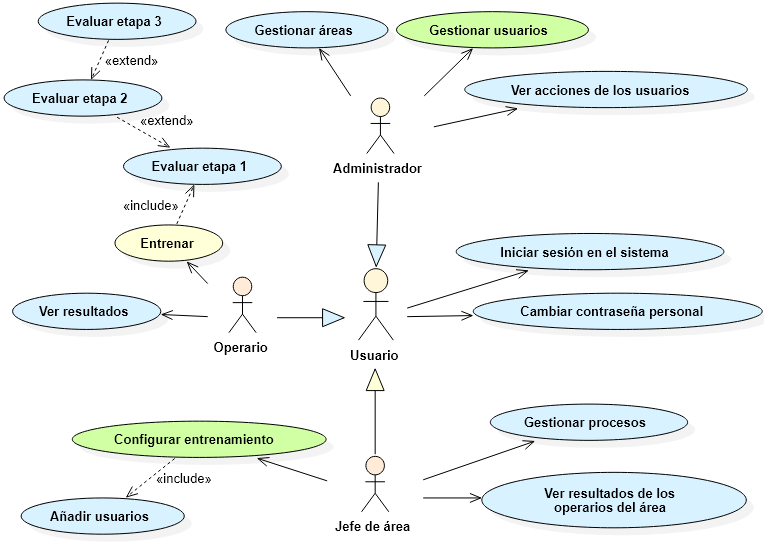
\includegraphics[width=0.65\linewidth]{imagen/dcu.png}
 \caption{Diagrama de casos de uso}
 \label{fig:dcu} 
\end{figure}

\subsection{Actores del sistema} 
Un actor puede referirse a cualquier entidad externa que interaccione con el sistema. No necesariamente coinciden con los usuarios. Un usuario puede interpretar distintos roles, correspondientes a distintos actores. Un actor puede desempeñar distintos papeles dependiendo del caso de uso en que participe \cite{Kalaivani2004}.

El Sistema Generador de Bases de Conocimiento (SGBC) es el encargado de confeccionar los ficheros de cada proceso dentro del sistema SECPROIT, como ya se explicó en el capítulo anterior. Sin embargo, este generador no se incluye como un actor, ya que no interactúa directamente con el sistema. Su relación es a partir de los ficheros que genera.

Los actores presentes en el nuevo sistema de capacitación (\textsl{Tabla \ref{tab:actores}}) están representados por tres roles: administrador, jefe de área u operario.

\begin{table}[H]
\begin{center}
\begin{tabular}{ | c | p{11cm} | }
\hline
\textbf{Actor} & \textbf{Descripción} \\
\hline
Usuario & Actor genérico que hace uso de las funcionalidades que son comunes \\
\hline
Operario & Actor que tiene acceso a los entrenamientos y posee un registro de sus resultados \\
\hline
Jefe de área & Actor que incluye los procesos a un área, decide cómo será el entrenamiento, qué usuarios podrán realizarlo y tiene acceso a los resultados de los operarios de su área \\
\hline
Administrador & Actor que gestiona las áreas, gestiona los usuarios y tiene acceso a un reporte de las acciones en el sistema \\
\hline
\end{tabular}
\caption{Actores del sistema}
\label{tab:actores}
\end{center}
\end{table}

\subsection{Especificación de los casos de uso}

\begin{table}[H]
\begin{center}
\begin{tabular}{ | c | p{3.5cm} |  p{7.5cm} |}
\hline
\textbf{Actor} & \textbf{Caso de uso} & \textbf{Descripción}\\
\hline
Administrador & Gestionar áreas & El actor puede introducir, modificar o eliminar las áreas del sistema \\
\cline{2-3}
& Gestionar usuarios & El actor puede introducir, modificar, dormir o activar a los usuarios del sistema \\
\cline{2-3}
& Ver acciones de los usuarios & El actor puede visualizar un registro con todas las acciones realizadas en el sistema \\
\hline
\end{tabular}
\caption{Casos de uso del administrador}
\end{center}
\end{table}

\begin{table}[H]
\begin{center}
\begin{tabular}{ | c | p{3.8cm} |  p{8cm} |}
\hline
\textbf{Actor} & \textbf{Caso de uso} & \textbf{Descripción}\\
\hline
Usuario & Iniciar sesión en el sistema & El actor debe introducir su nombre de usuario y su contraseña para iniciar sesión en el sistema \\
\cline{2-3}
& Cambiar contraseña personal  & El actor puede cambiar la contraseña que posee por defecto, por una de su preferencia \\
\hline
\end{tabular}
\caption{Casos de uso del usuario}
\end{center}
\end{table}

\begin{table}[H]
\begin{center}
\begin{tabular}{ | c | p{3cm} |  p{8.5cm} |}
\hline
\textbf{Actor} & \textbf{Caso de uso} & \textbf{Descripción}\\
\hline
Operario & Entrenar & El actor inicia el entrenamiento de un proceso \\
\cline{2-3}
& Entrenar en la primera etapa & El actor se evalúa en la primera etapa del entrenamiento (debe escoger las variables que se encuentran fuera de rango) \\
\cline{2-3}
& Entrenar en la segunda etapa & El actor se evalúa en la segunda etapa del entrenamiento (debe escoger las causas de las variables que se encuentran fuera de rango) \\
\cline{2-3}
& Entrenar en la tercera etapa & El actor se evalúa en la tercera etapa del entrenamiento (debe escoger las recomendaciones de las causas) \\
\cline{2-3}
& Ver resultados & El actor puede visualizar un registro con todos los resultados que ha obtenido \\
\hline
\end{tabular}
\caption{Casos de uso del operario}
\end{center}
\end{table}

\begin{table}[H]
\begin{center}
\begin{tabular}{ | c | p{3.5cm} |  p{7.5cm} |}
\hline
\textbf{Actor} & \textbf{Caso de uso} & \textbf{Descripción}\\
\hline
Jefe de área & Gestionar procesos & El actor puede introducir, modificar o eliminar los procesos de su área \\
\cline{2-3}
& Configurar entrenamiento & El actor decide para cada proceso cómo será el entrenamiento \\
\cline{2-3}
& Añadir usuarios & El actor decide para cada proceso los usuarios que lo pueden realizar \\
\cline{2-3}
& Ver resultados de los operarios del área & El actor puede visualizar un registro con todas las evaluaciones de los operarios de su área \\
\hline
\end{tabular}
\caption{Casos de uso del jefe de área}
\end{center}
\end{table}

\section{Modelo de datos}
Para el desarrollo de este sistema se utiliza, como gestor de base de datos, la herramienta PostgreSQL. En ella se almacena toda la información con la que se va a trabajar, incluyendo los ficheros \textsl{anm} y \textsl{drl} de los procesos. Por momentos determinados, esta información también se encuentra almacenada, de forma local y temporal, en clases del propio sistema, lo que permite un mejor manejo y control de los datos.

\subsection{Diagrama de Entidades y Relaciones (DER)}
Un Diagrama de Entidades y Relaciones (DER) es una herramienta que permite representar de manera simplificada los componentes que participan en un proceso, y el modo en el que estos se relacionan entre sí. Posee tres elementos principales: las entidades, los atributos y las relaciones \cite{Li2009}.

El diagrama de entidades de este nuevo sistema de capacitación (\textsl{Figura \ref{fig:der}}) contiene varias modificaciones con respecto al diagrama presente en el sistema SECPROIT. Para una mejor representación de los cambios, se tuvieron en cuenta una serie de colores:

\begin{itemize}
\item \textbf{Azul}: representa aquellas entidades que no sufrieron ningún cambio significativo con respecto al sistema SECPROIT
\item \textbf{Amarillo}: representa aquellas entidades que fueron modificadas, pero que siguen cumpliendo las mismas funciones
\item \textbf{Verde}: representa las entidades que son totalmente nuevas
\end{itemize}

\begin{figure}[h]
\centering
 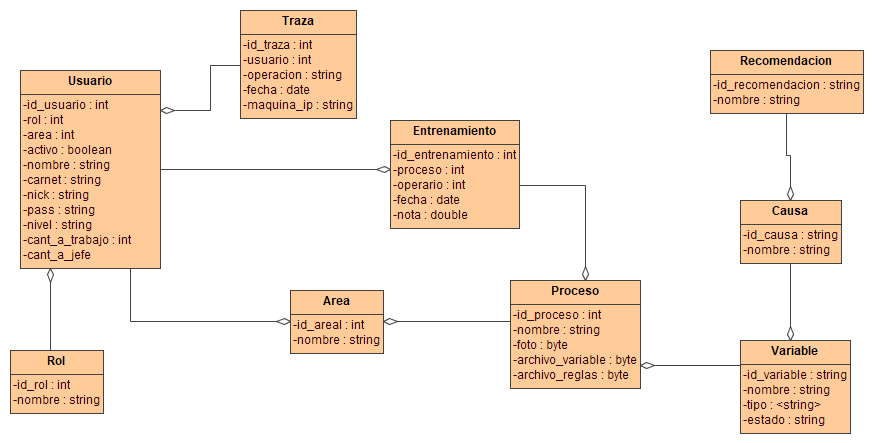
\includegraphics[width=0.65\linewidth]{imagen/der.png}
 \caption{Diagrama de Entidades y Relaciones (DER)}
 \label{fig:der} 
\end{figure}

En este diagrama no solo se cambiaron y se agregaron nuevas entidades, también se eliminaron algunas de las entidades presentes en el diagrama del sistema SECPROIT, debido a que ya no eran necesarias su funciones. Para realizar una comparación más detallada puede verse \cite{ElenaAcostaGil2018}, donde se encuentra el diagrama mencionado junto a su explicación. Las modificaciones realizadas (\textsl{Tabla \ref{tab:entidades}}) se hicieron con el fin de resolver algunas de las limitaciones presentes en el SECPROIT.

\begin{table}[H]
\centering
\begin{center}
\begin{tabular}{ | c | p{5cm} |  p{5cm} | }
\hline
\textbf{Entidad} & \textbf{Atributos}  & \textbf{Descripción}\\
\hline
Área & ID y nombre & No sufrió ningún cambio \\
\cline{1-2}
Traza & ID, usuario, acción y fecha &  \\
\cline{1-2}
Proceso & ID, nombre, foto, base de datos, base de reglas y área &  \\
\hline
Usuario & ID, nombre, carnet, nivel escolar, experiencia, años como jefe, usuario, contraseña, área, rol y activo & Se agregaron nuevos atributos que permiten conocer mejor al usuario\\
\hline
Configuración & ID, proceso, tiempo, cantidad de preguntas, cantidad de preguntas aprobadas y tipos de pregunta & Se agregó con el fin de poder configurar los entrenamientos \\
\hline
Entrenamiento & ID, operario, configuración de proceso, cantidad de intentos, cantidad de intentos aprobados, primera etapa, segunda etapa, tercera etapa y nota general & Se eliminaron los demás atributos que poseía \\
\hline
Etapa-Entrenamiento & ID, entrenamiento, tipo de etapa, tiempo, preguntas acertadas y nota & Se agregó para poder tener una pausa entre etapas y poder realizar más de una prueba por etapa \\
\hline
Variable & ID, nombre, tipo, valor mínimo, valor máximo y proceso & Se agregó en el sistema para agilizar el proceso de lectura \\
\cline{1-2}
Causa & ID y nombre &  \\
\cline{1-2}
Recomendación & ID y nombre & \\
\cline{1-2}
Variable-Causa & ID, variable y causa &  \\
\cline{1-2}
Causa-Recomendación & ID, causa y recomendación &  \\
\hline
\end{tabular}
\caption{Entidades del nuevo sistema de capacitación}
\label{tab:entidades}
\end{center}
\end{table}

\subsection{Diagrama de base de datos}
La herramienta utilizada para crear y gestionar la base de datos del nuevo sistema de capacitación (PostgreSQL), permite exportar un diagrama de la misma (\textsl{Figura \ref{fig:bd}}). En dicho diagrama se pueden apreciar las relaciones existentes entre las entidades del software y los atributos que poseen cada una.

\begin{figure}[H]
\centering
 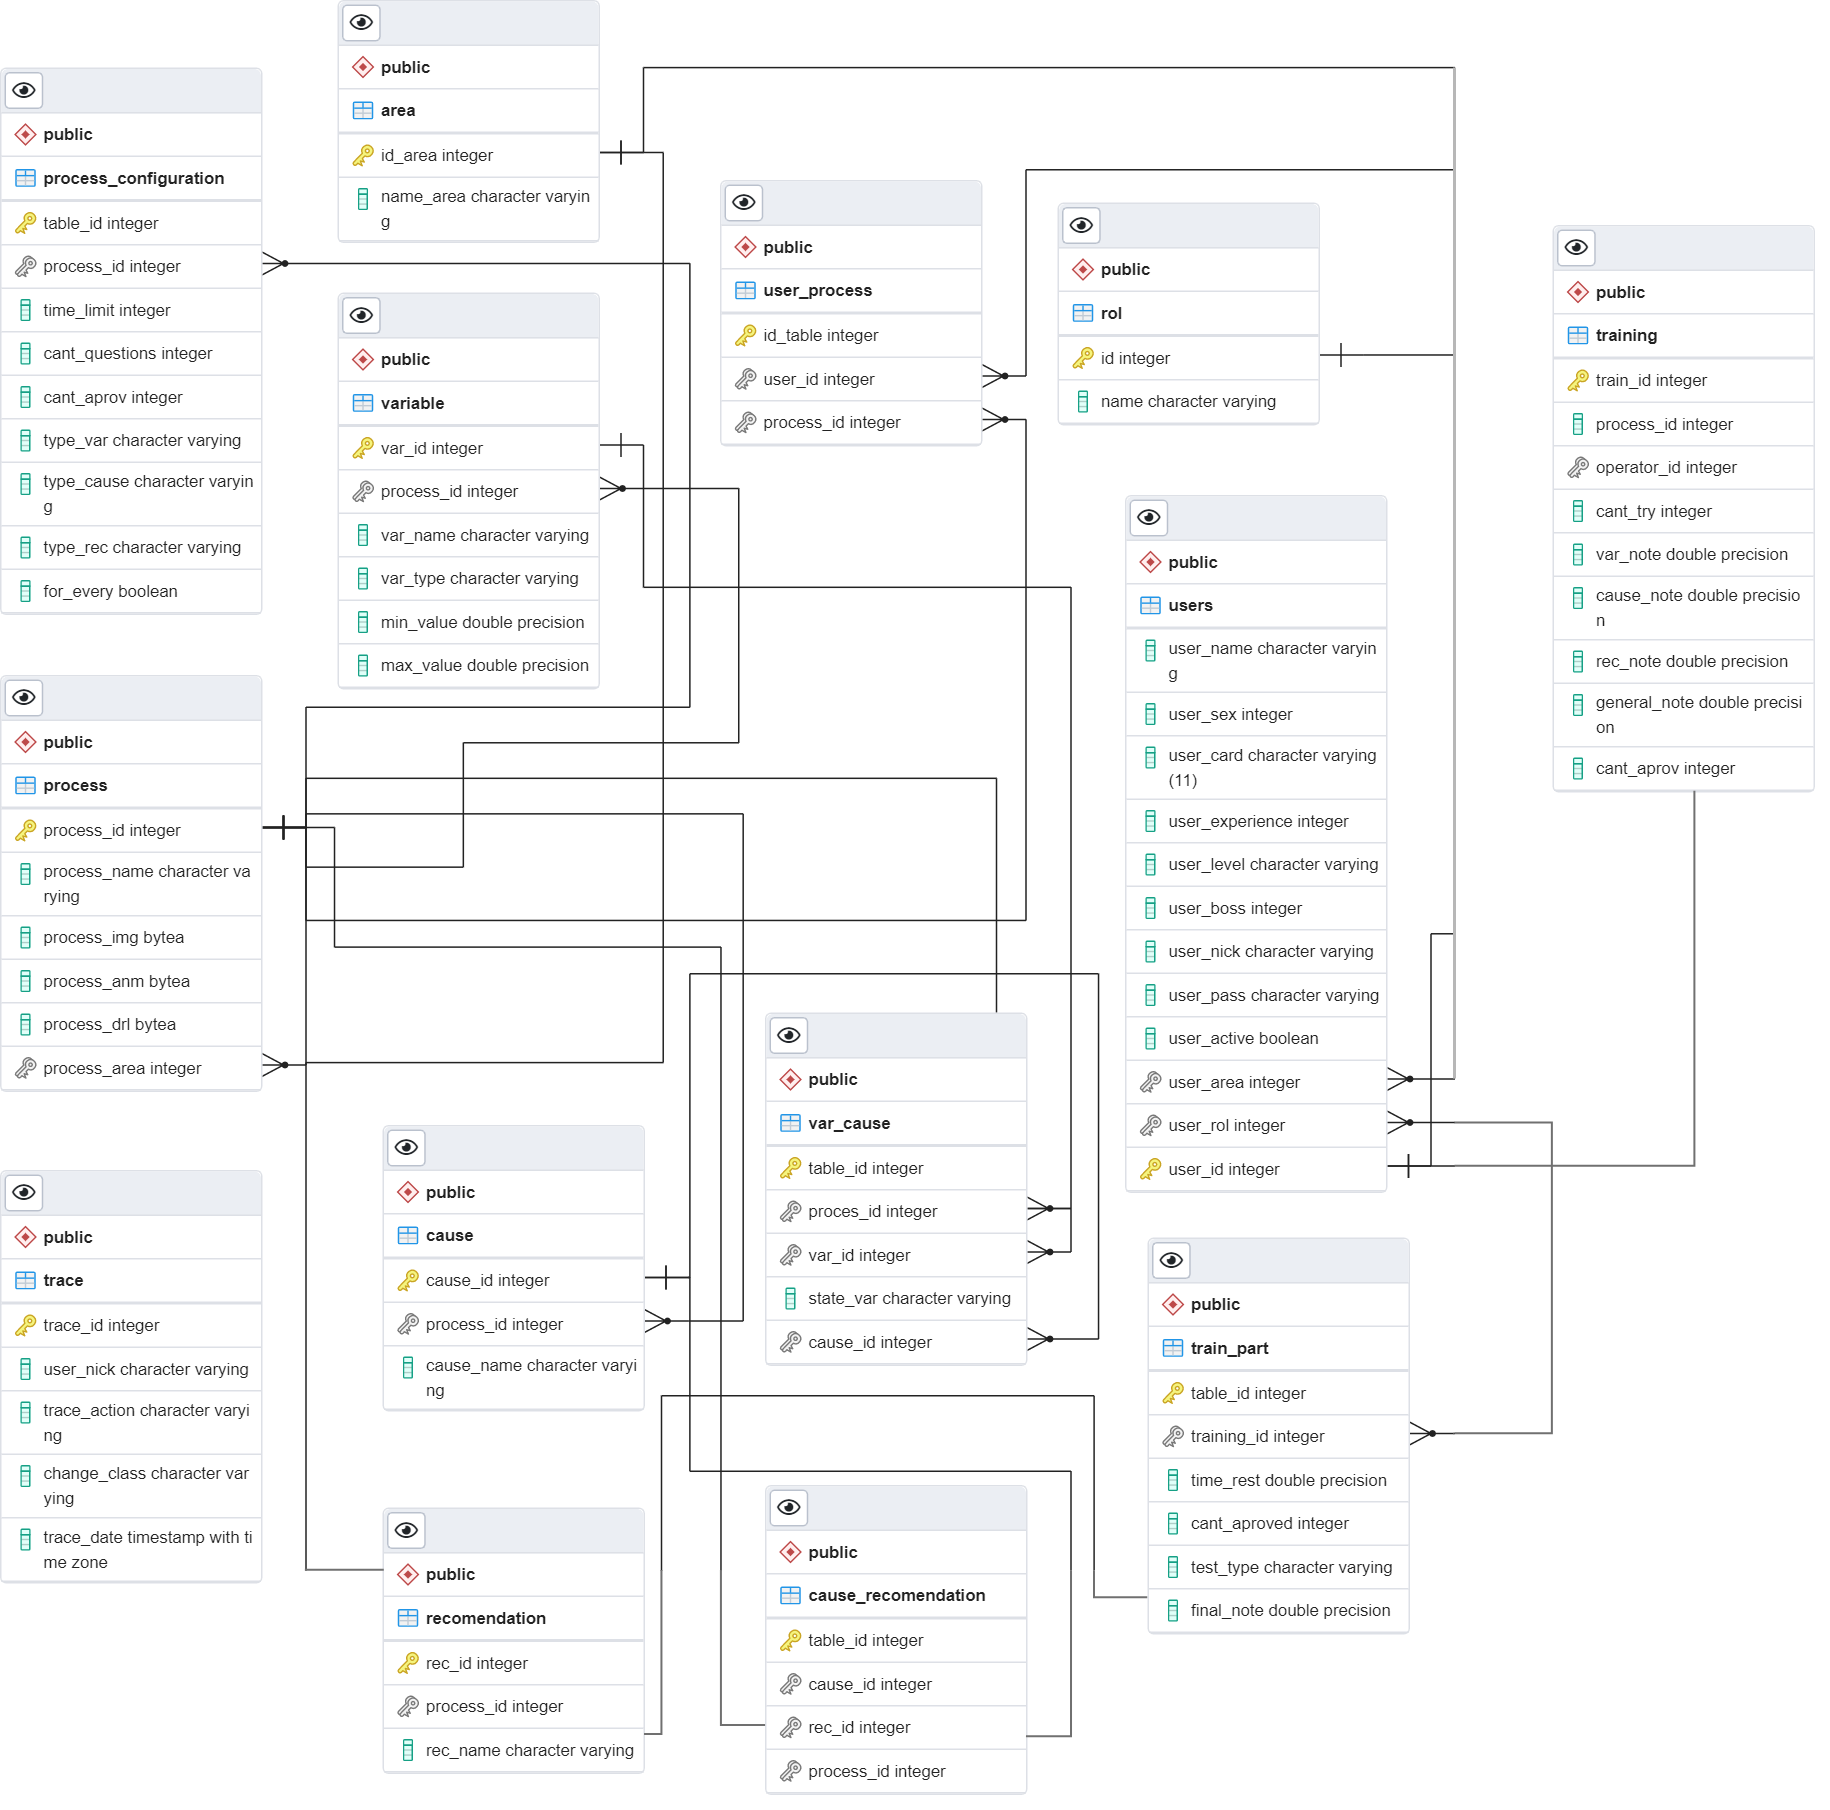
\includegraphics[width=0.9\linewidth]{imagen/bd.png}
 \caption{Diagrama de base de datos}
 \label{fig:bd} 
\end{figure}

\section{Arquitectura de paquetes del nuevo sistema de capacitación}
El patrón arquitectónico de capas ayuda a estructurar las aplicaciones, organizando las clases en grupos de subtareas, en donde que cada uno se encuentra a un nivel particular de abstracción. Se basa en una distribución jerárquica de los roles y las responsabilidades, para proporcionar una división efectiva de los problemas a resolver. Los roles indican el tipo y la forma de la interacción con otras capas y las responsabilidades, la funcionalidad que implementan \cite{Plecka2013}.

En este nuevo sistema de capacitación, se crearon un conjunto de paquetes  (\textsl{Tabla \ref{tab:paquetes}})  que agrupan las clases del sistema. Cada paquete responde a una funcionalidad o a una estructura específica, para ayudar con la organización del proyecto.

\begin{figure}[H]
\centering
 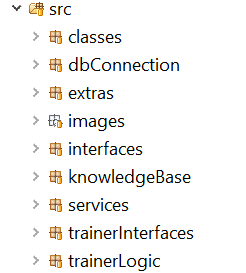
\includegraphics[width=0.27\linewidth]{imagen/paquetes.png}
 \caption{Arquitectura de los paquetes de clases}
 \label{fig:paquetes} 
\end{figure}

\begin{table}[H]
\centering
\begin{center}
\begin{tabular}{ | c | p{11.5cm} | }
\hline
\textbf{Paquete} & \textbf{Descripción}\\
\hline
classes & Contiene las clases que representan las entidades registradas en la base de datos \\
\hline
dbConnection & Contiene las clases que permiten establecer una conexión con la base de datos \\
\hline
extras & Contiene las clases que auxilian el proceso de generar las interfaces del sistema y clases que poseen funciones de validación \\
\hline
images & Contiene las imágenes utilizadas en el sistema \\
\hline
interfaces & Contiene las interfaces visuales del sistema \\
\hline
knowledgeBase & Contiene las clases que permiten establecer una conexión con el \textsl{JDrools}, así como las clases que auxilian el proceso de cargar y leer un fichero (todo lo relacionado con el sistema experto) \\
\hline
services & Contiene las clases que brindan un servicio a la base de datos (insertar, leer, modificar o eliminar) \\
\hline
trainerInterfaces & Contiene las interfaces visuales relacionadas con las etapas del entrenamiento \\
\hline
trainerLogic &  Contiene las clases que permiten el correcto funcionamiento de una etapa de entrenamiento \\
\hline
\end{tabular}
\caption{Descripción de los paquetes de clases}
\label{tab:paquetes}
\end{center}
\end{table}

\section{Proceso de entrenamiento}
Los entrenamientos están compuestos por tres etapas: variables, causas y recomendaciones. Cada etapa es decisiva en la evaluación final del entrenamiento, por lo tanto, se deben aprobar todas las etapas para afirmar que un entrenamiento fue completado. De lo contrario, el operario será notificado como suspenso en ese proceso.

Una de las funcionalidades presentes en el nuevo sistema de capacitación es la configuración de entrenamiento. Gracias a esta, un operario puede realizar varios intentos en una misma etapa, acumulando puntos positivos a su promedio, es decir, si suspende, tiene la oportunidad de volverlo a intentar. También se incluyeron nuevos tipos de preguntas, lo que aumenta el método de aprendizaje del adiestrado. 

Las preguntas de cada etapa se generan de forma aleatoria, incluyendo entrenamientos con todas las preguntas correctas o todas incorrectas. De esta manera se evita el fraude y el aprendizaje por memoria.

\subsection{Modelo matemático de la evaluación por etapas}
En el sistema SECPROIT, para evaluar una etapa se utiliza un método de evaluación por escala, es decir, dependiendo de la cantidad de preguntas acertadas se devuelve una evaluación de acuerdo a la escala que se tiene (muy mal, mal, regular, bien, muy bien y excelente). El sistema que utiliza para mostrar los resultados es el sistema de aprobado o no, dejando en claro el nivel de satisfacción según la escala mencionada anteriormente.

Este tipo de evaluación trae como resultado la desinformación del usuario, ya que no se puede apreciar a simple vista la evolución del mismo. Por esa razón, es necesario establecer un sistema numérico que permita observar el avance del operario.

En el nuevo sistema de capacitación se insertó un sistema de evaluación a base de fórmula, tomando en cuenta los parámetros de: tiempo y cantidad de preguntas correctas. El parámetro del tiempo, en este tipo de evaluación, es decisivo, porque el objetivo de este sistema es preparar a los operarios para situaciones reales y, en las industrias, mientras más rápido se resuelva una falla, menores problemas y daños ocasiona.

La fórmula utilizada en el nuevo sistema de capacitación es:

\vspace{0.2cm}
\begin{center}
\begin{Large}
\textbf{N} = (Ca/C + (Td/T \cdot  0.1))
\end{Large}
\end{center}
\vspace{0.15cm}

Donde \textbf{N} es la calificación obtenida en la etapa, \textbf{Ca} es la cantidad de preguntas acertadas, \textbf{C} es la cantidad de preguntas en total, \textbf{Td} es el tiempo demorado en responder todas las preguntas (en minutos) y \textbf{T} es el tiempo total (en minutos). Nótese que el tiempo es multiplicado por 0,1. Esto se debe a que el valor del tiempo es importante, pero no debe ser tomado como requisito fundamental, es decir, afecta la evaluación, pero no influye en el aprobado o desaprobado de la misma \cite{Castrillon2021}.

\subsection{Modelo matemático de la evaluación general}
En el sistema SECPROIT no existe la evaluación general de un entrenamiento. Por cada etapa se tiene una escala (muy mal, mal, regular, bien, muy bien y excelente) y a partir de esta se determina si el usuario aprobó o no.

En el nuevo sistema de capacitación se incorporó una fórmula para calcular la evaluación final de un entrenamiento a partir del promedio de las notas obtenidas por el usuario en cada una de las etapas. De esta manera se puede realizar un estudio más profundo y detallado de las habilidades de los operarios, así como extraer estadísticas generales con las notas de los usuarios.

La fórmula utilizada para obtener el resultado final del entrenamiento de un proceso es la siguiente:

\vspace{0.15cm}
\begin{center}
\begin{Large}
\textbf{Ng} = (E1 \cdot 0.4) + (E2 \cdot  0.3) + (E3 \cdot  0.3)
\end{Large}
\end{center}
\vspace{0.15cm}

Donde \textbf{Ng} es la calificación general del entrenamiento, \textbf{E1} es el promedio de las evaluaciones aprobadas de la etapa 1, \textbf{E2} es el promedio de las evaluaciones aprobadas de la etapa 2 y \textbf{E3} es el promedio de las evaluaciones aprobadas de la etapa 3. Nótese que el primer promedio se multiplica por 0,4 y los otros dos se multiplica por 0,3. Esto se debe a que el valor del resultado final es en base a 10 y a que la primera etapa (variables) es más extensa y más difícil que las otras dos etapas (causas y recomendaciones).

\section{Interfaces de usuario}

\section{Conclusiones parciales}
